\documentclass{article}%
\usepackage[T1]{fontenc}%
\usepackage[utf8]{inputenc}%
\usepackage{lmodern}%
\usepackage{textcomp}%
\usepackage{lastpage}%
\usepackage[head=40pt,margin=0.5in,bottom=0.6in]{geometry}%
\usepackage{graphicx}%
%
\title{\textbf{La mayoría de las empresas no se acogió al subsidio de Maduro}}%
\author{CARLOS SEIJAS MENESES | cseijas@el{-}nacional.com}%
\date{18/10/2018}%
%
\begin{document}%
\normalsize%
\maketitle%
\textbf{URL: }%
http://www.el{-}nacional.com/noticias/economia/mayoria{-}las{-}empresas{-}acogio{-}subsidio{-}maduro\_256225\newline%
%
\textbf{Periodico: }%
EN, %
ID: %
256225, %
Seccion: %
Economía\newline%
%
\textbf{Palabras Claves: }%
NO\_TIENE\newline%
%
\textbf{Derecho: }%
2.3%
, Otros Derechos: %
NO\_TIENE%
, Sub Derechos: %
2.3.1%
\newline%
%
\textbf{EP: }%
NO\newline%
\newline%
%
\textbf{\textit{El nuevo Dicom ha otorgado 35,3 millones de dólares al sector privado, cuando se requieren 120 millones diarios para satisfacer niveles de demanda de 2014}}%
\newline%
\newline%
%
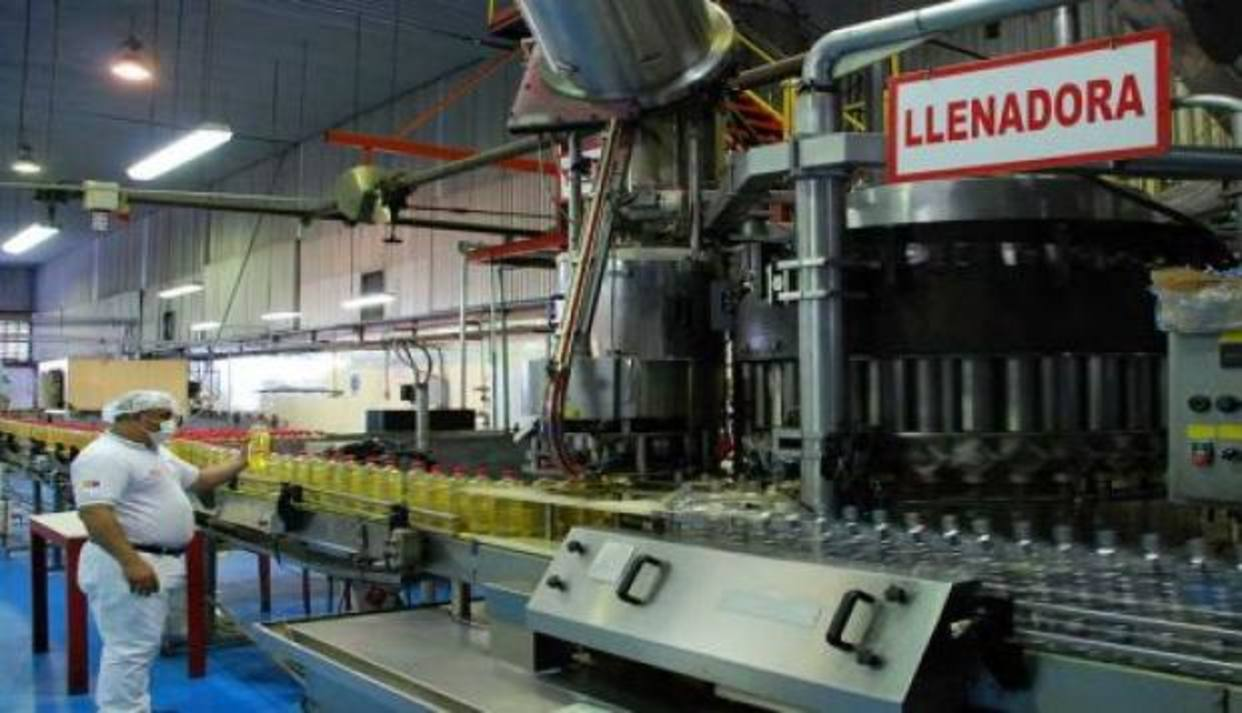
\includegraphics[width=300px]{155.jpg}%
\newline%
%
En los 58 días que han pasado del Programa de Recuperación Económica, el gobierno asegura que cumplió con el pago de las nóminas del sector privado y que les dio a los empresarios materia prima, créditos en bolívares y 200 millones de dólares para importaciones. “¿Qué quieren, qué les haga el muchacho y se lo para también?”, expresó el presidente Nicolás Maduro.%
\newline%
%
Pero la realidad contradice lo dicho por el mandatario. Dirigentes empresariales afirman que el grueso de las compañías privadas decidió no aceptar al subsidio que el gobierno ofreció, además de que la oferta de divisas y de materia prima ha sido insuficiente.%
\newline%
%
Juan Pablo Olalquiaga, presidente de~la Confederación Venezolana~de Industriales, declaró que la mayoría de las empresas no se acogió al subsidio. “Pero el gobierno hizo depósitos en las cuentas de muchos trabajadores porque sí, a la fuerza, sin petición, sin presupuesto y sin estructura jurídica ni legislativa que sustente tales depósitos”, dijo.%
\newline%
%
Carlos Larrazábal, presidente de Fedecámaras, coincidió con Olalquiaga. Afirmó que en las consultas del gremio con sus cámaras afiliadas se demostró que la mayoría de las empresas asumió el compromiso del ajuste del salario, que Maduro aumentó de~30 a~1.800 bolívares soberanos.%
\newline%
%
“Hay información cruzada referida a que algunos trabajadores se registraron en la página del gobierno y con el carnet de la patria recibieron algún tipo de bonificación directa, pero eso no significa que haya pagado la nómina de las empresas”.%
\newline%
%
Indicó que a algunos productores el gobierno les ha vendido a precios de mercado determinadas materias primas básicas que importó como maíz, sorgo, trigo y azúcar cruda, pero no es suficiente para las necesidades del consumo. “No ha sido una dádiva sino una operación de venta en vista de que el gobierno no permite que las empresas importen directamente y que no hay disponibilidad de divisas para que esa adquisición se pueda hacer”, explicó el empresario.%
\newline%
%
En las 23 subastas que ha realizado el nuevo Dicom, desde que entró en vigencia el plan económico gubernamental, ha otorgado un total de 35.394.413,22 de dólares a las empresas. Debido a la destrucción de las fuentes de materia prima, las compañías necesitarían cerca de 120 millones de dólares diarios para satisfacer los niveles de demanda de 2014, según cálculos de Conindustria.%
\newline%
%
“Los dólares no están”, aseguró Olalquiaga. El total adjudicado por el Dicom entre agosto y septiembre, dividido entre las 3.200 empresas que quedan en el país, no alcanza para nada, aseveró.%
\newline%
%
Una industria normalmente requiere, por lo menos, 1.000 SKU (ítem) para operar, que pueden ser trigo, papel para facturar o una correa dentada. “Si a una empresa que produce alimentos el gobierno le dio trigo, está bien, pero con eso por sí solo no funciona una fábrica. Esa percepción simplista que el Ejecutivo tiene de que les dio a las empresas todo lo que les hacía falta para trabajar es una demostración más de ignorancia que de compresión de lo complejo que es un proceso industrial”, añadió Olalquiaga.%
\newline%
%
\end{document}